\section{数据检索}
\subsection{打开网站}
\begin{frame}{打开浏览器}
    打开一个非IE浏览器,以火狐为例。
    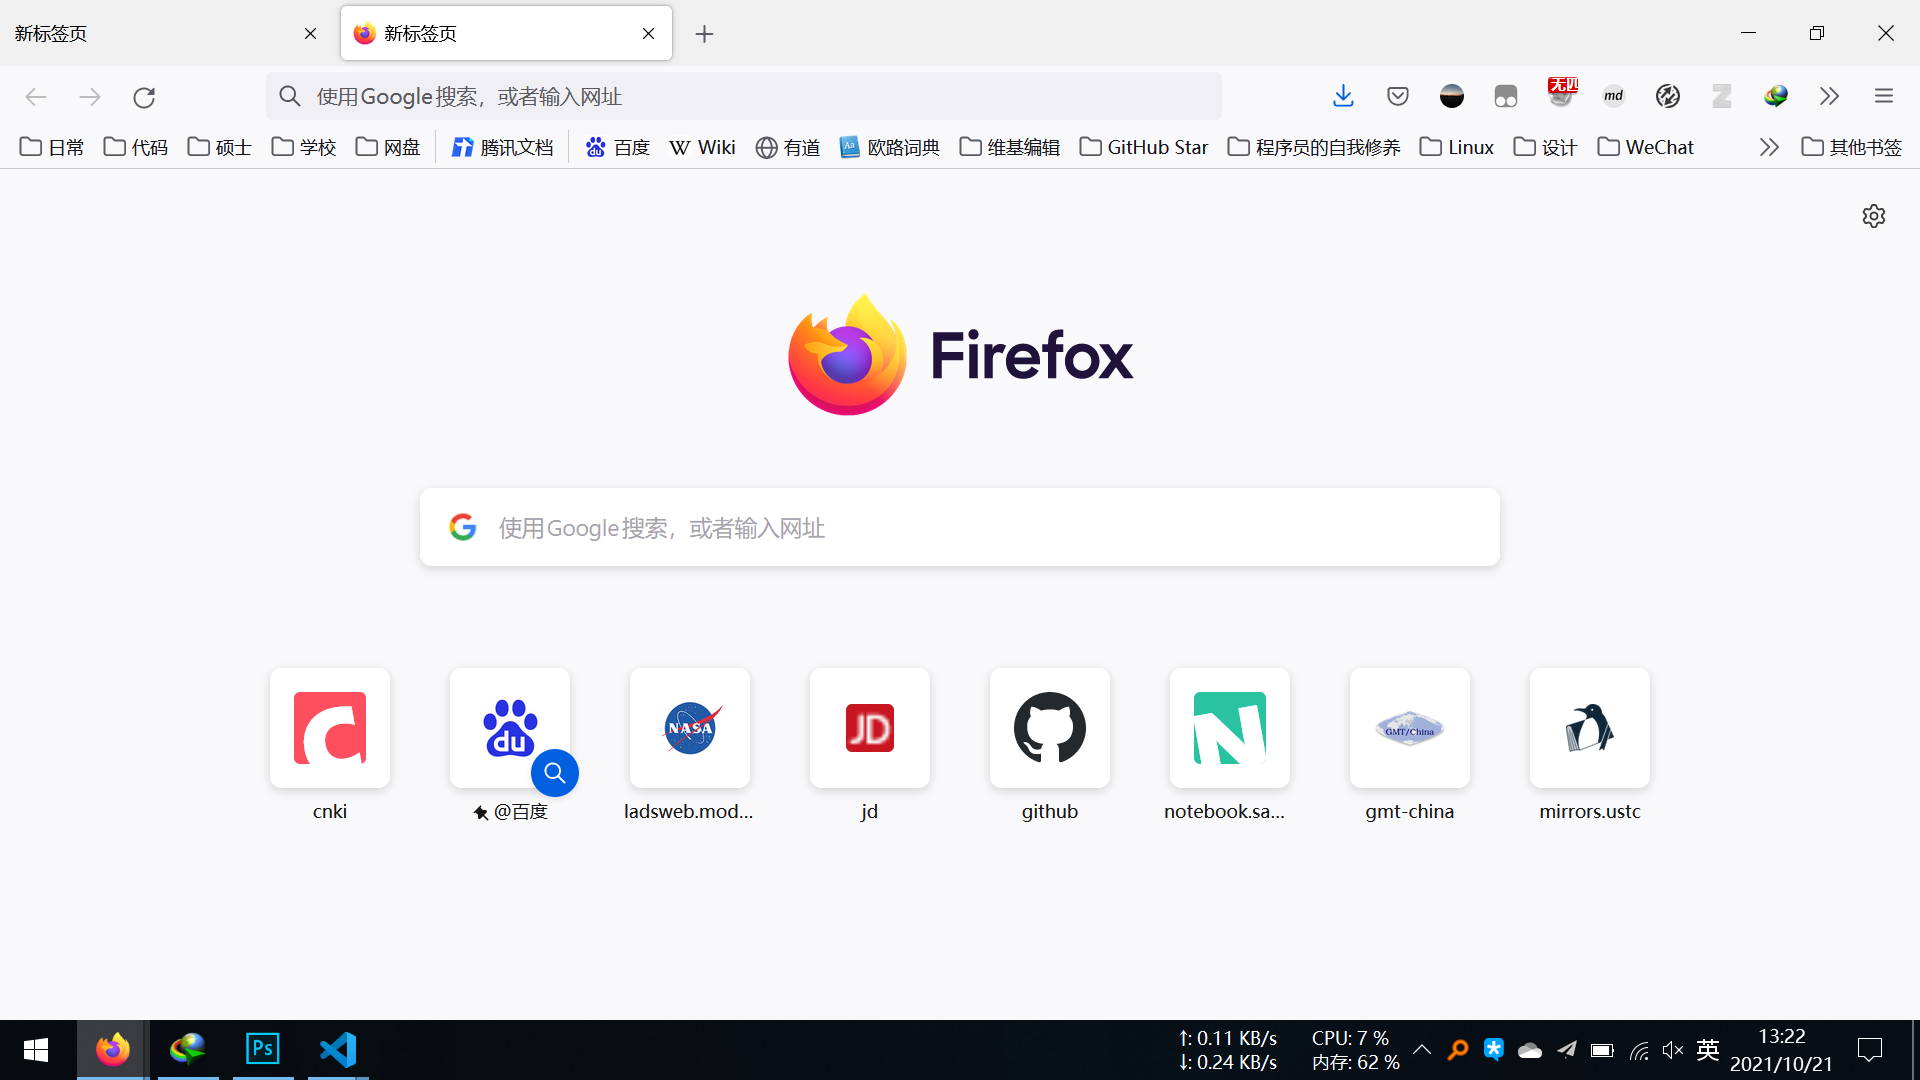
\includegraphics[width=\linewidth]{images/1.打开浏览器.png}
\end{frame}
\begin{frame}
    \frametitle{输入LAADS网址}
    输入网址\url{https://ladsweb.modaps.eosdis.nasa.gov/}

    按键盘上的Enter键或鼠标点击访问。
    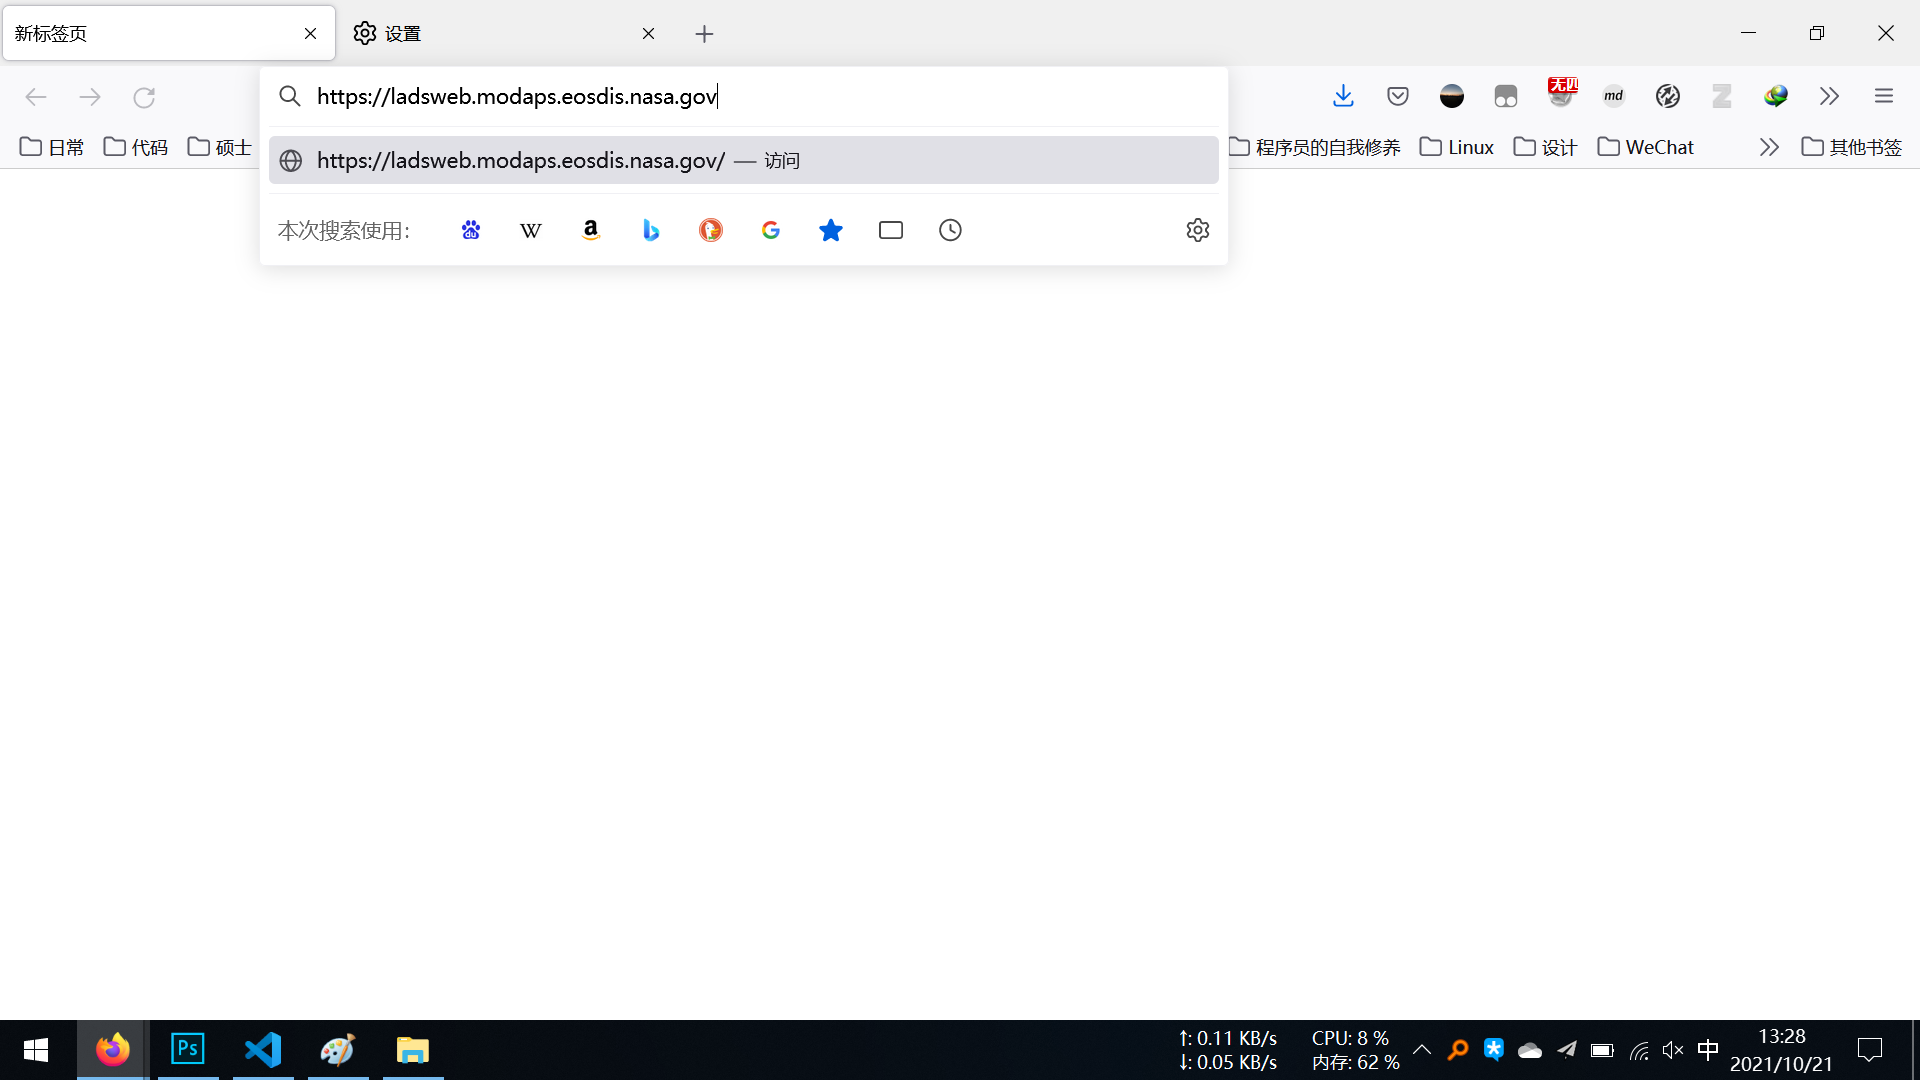
\includegraphics[width=\linewidth]{images/2.输入LAADS网址.png}
\end{frame}
\begin{frame}
    \frametitle{打开登录界面}
    点右上角的\uline{Profile},然后点击\uline{Earthdata Login}
    \begin{annotationimage}{width=\linewidth}{images/3.找到登录入口.png}
        \draw[red,very thick] (0.855,0.71) -- (0.997,0.71) -- (0.997,0.95) --(0.925,0.95) -- (0.925,0.82) -- (0.855,0.82) -- cycle;
    \end{annotationimage}
\end{frame}
\subsection{注册帐号}
\begin{frame}
    \frametitle{登录/注册}
    有账号直接输入点\uline{LOGIN IN}登录,没帐号点\uline{REGISTER}注册先

    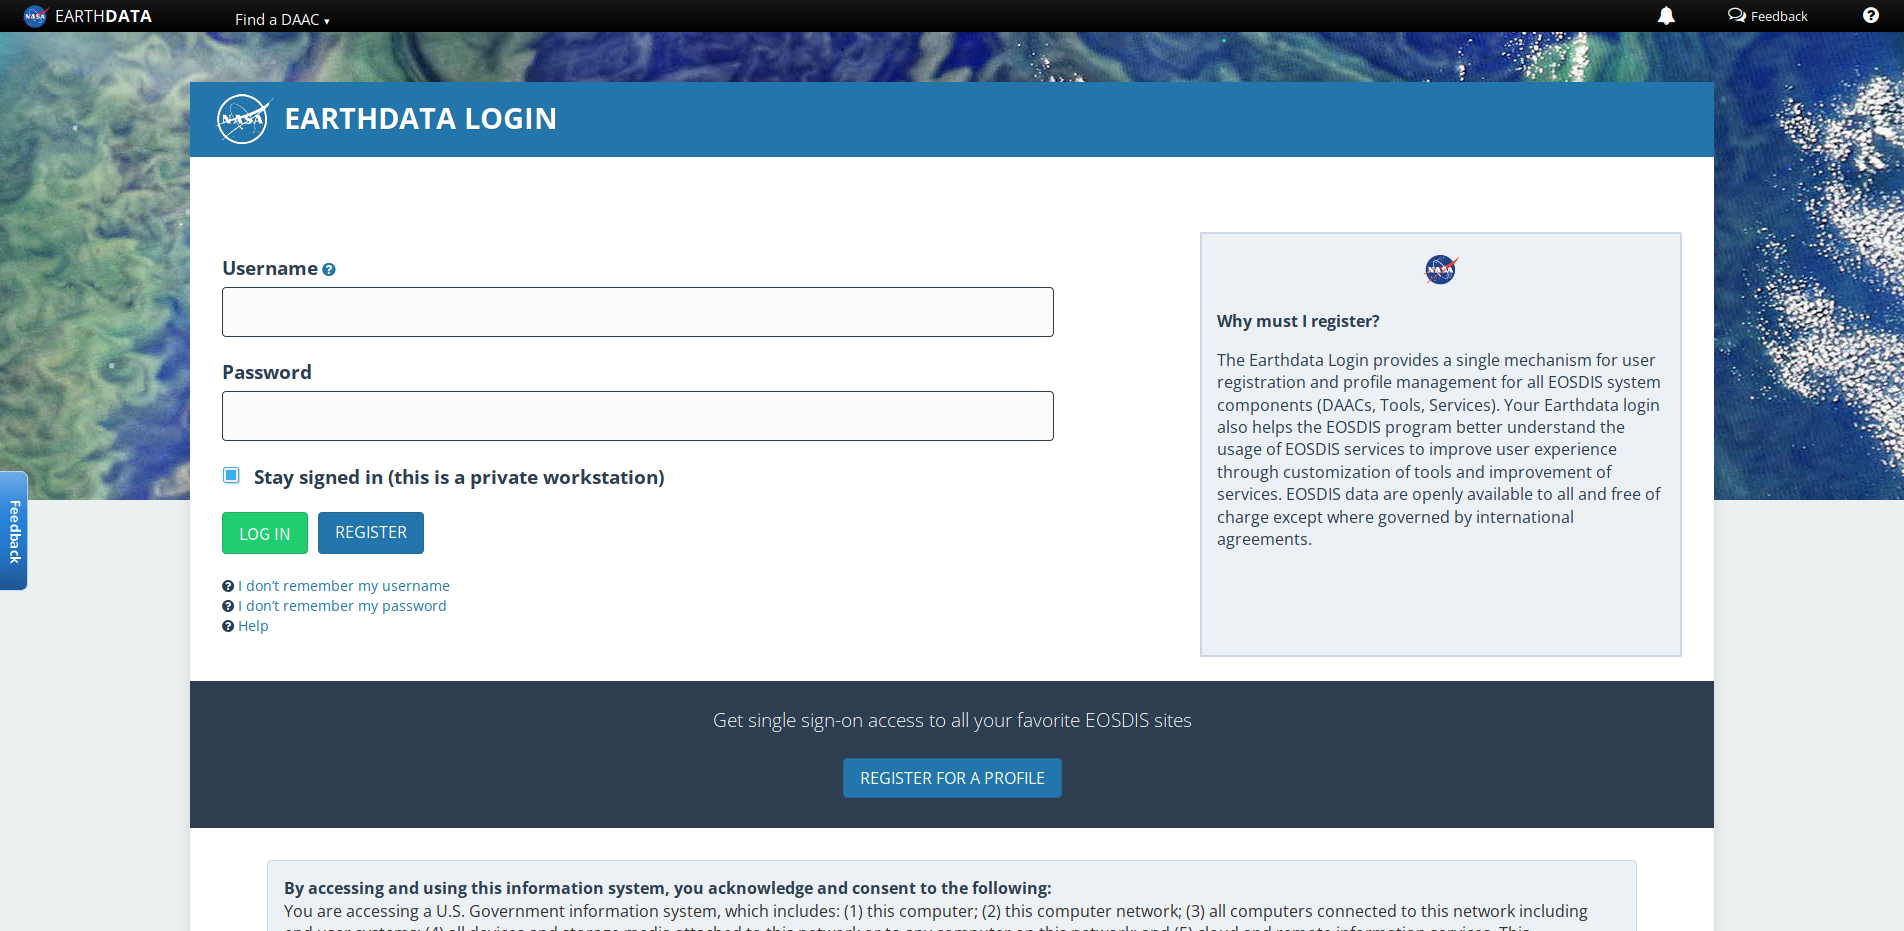
\includegraphics[width=\linewidth]{images/4.登陆界面.png}

    假设你没帐号
    % \begin{annotationimage}{width=\linewidth}{images/4.登陆界面.png}
    % \draw[red,very thick] (0.115,0.4) -- (0.165,0.4) -- (0.165,0.46) -- (0.115,0.46) -- cycle;
    % \draw[coordinate label = {登录点这里 at (0.14,0.34)}];
    % \draw[annotation left={登录点这 at 0.3}] to (0.15,0.41);
    % \draw[annotation below={注册点这 at 0.3}] to (0.2,0.45);
    % \end{annotationimage}
\end{frame}
\begin{frame}
    \frametitle{填信息}
    按要求填写标红星的选项
    \footnote{QQ邮箱也可以}
    ;底部的Agreements内容全选

    点击底部\uline{Register for Earthdata Login}确认注册
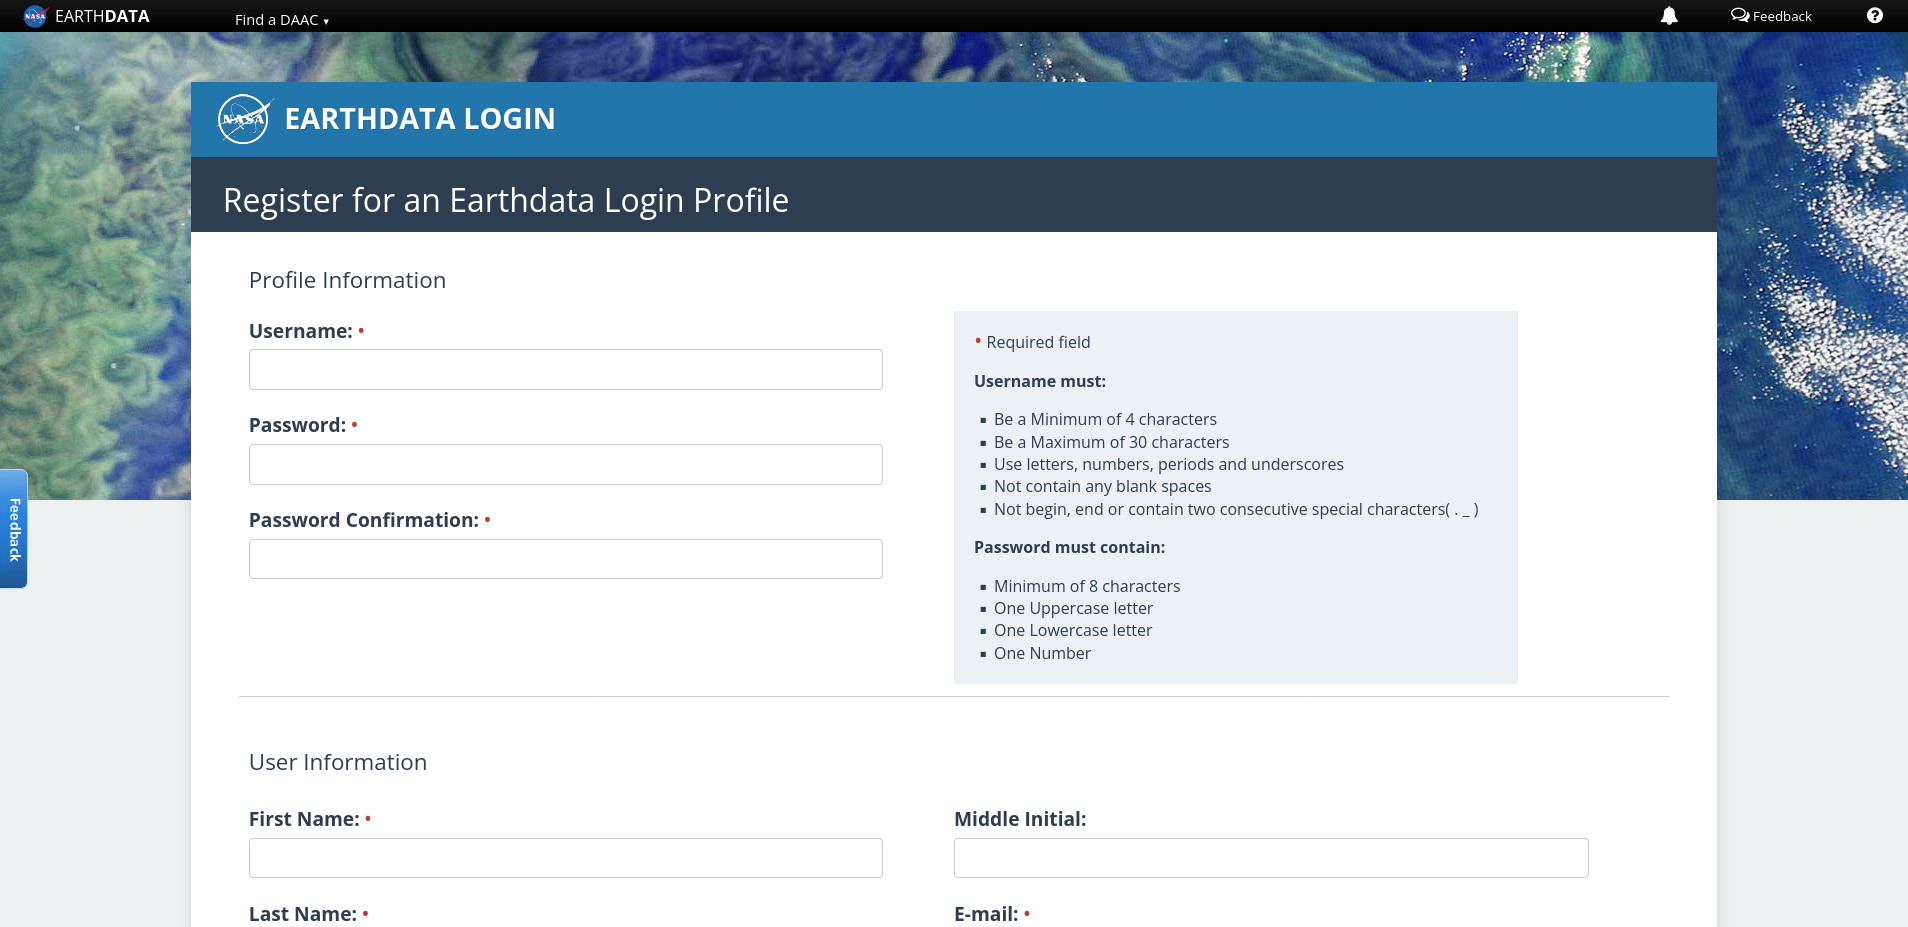
\includegraphics[width=\linewidth]{images/5.注册帐号.png}
\end{frame}
\begin{frame}
    \frametitle{登录}
    注册完回来,输入你注册的用户名和密码,登录
    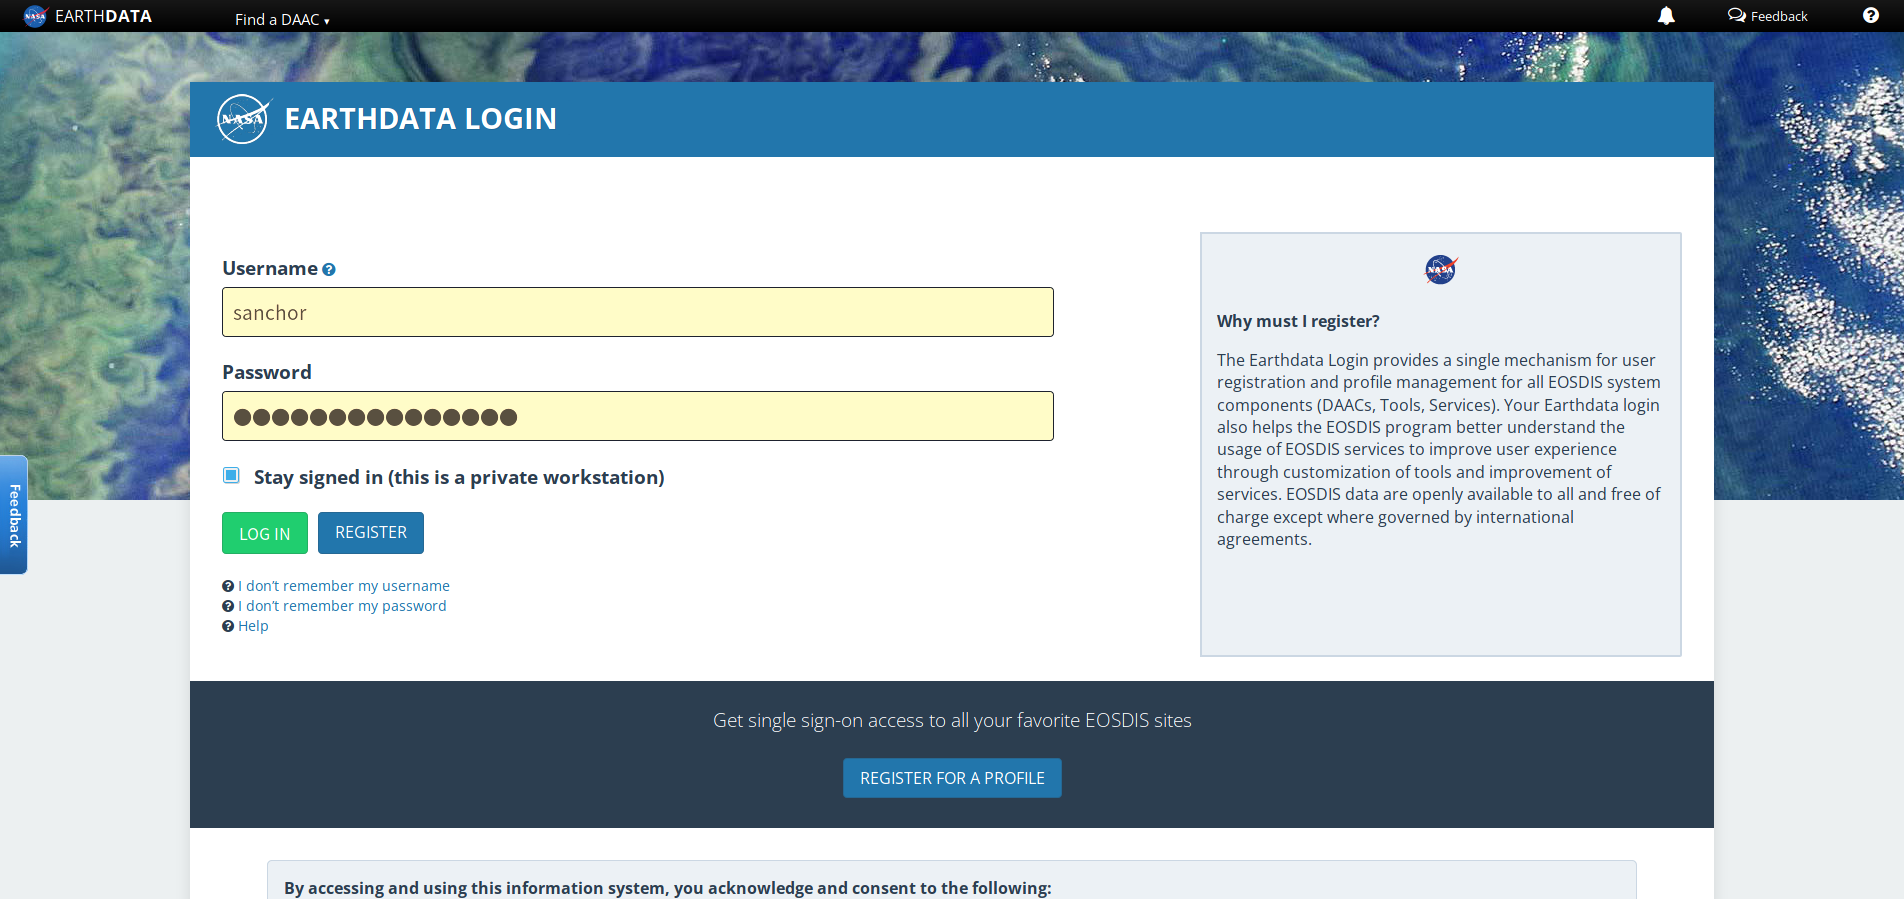
\includegraphics[width=\linewidth]{images/7.登录.png}
\end{frame}
\begin{frame}
    \frametitle{登录完成}
    登录完会返回主页,再点击右上角的\uline{Profile}会不一样
 \begin{annotationimage}{width=\linewidth}{images/8.登录完成.jpg}
    \draw[red,very thick] (0.87,0.74) -- (0.997,0.74) -- (0.997,0.97) --(0.945,0.97) -- (0.945,0.9) -- (0.87,0.90) -- cycle;
\end{annotationimage}
\subsection{执行检索}
\subsection{提交订单}
\end{frame}